\begin{multicols}{3}
\byline{Europe go green - Какво, с кого, как и дали си струва?}{Силвия Мечкова и Атанас Атанасов, Х "а" клас}

Какво е "Europe go green" ? 

"Europe go green" е екологичен проект, организиран по проекта "Коменски" с цел обогатяване и развиване на знанията на учениците по екология и опазване на околната среда. В този проект ние не само добиваме знания, но и провеждаме инициативи, с които искаме да запознаем и околните с дейността си. В проекта участват ГПНЕ "Гьоте" заедно с гимназия "Хумболдт" в гр. Гифхорн, Германия,  гимназия номер 2 в гр. Реда, Полша, Езиков лицей в гр. Л'Аквила, Италия и Дъмфри Академия, гр. Дъмфри, Шотландия.

Как се развива дейноста от началото на проекта до сега?

Началото на проекта бе поставено още през 2012 година, когато се проведе проучване между заинтересованите от екология ученици, които избраха за тема на проекта "Водата". 

През месец октомври 2012г. се проведоха регуларни срещи между петимата участници и техните учители и ръководители в проекта - г-жа Светлана Вичева и г-жа Весела Христова. Тогава бе изработен и изпратен "Mind map" до първия ни домакин в гр. Реда, Полша.През месец ноември се проведе и първата среща в гр.Реда, където участниците представиха папките си. Деница Ковачева направи проби на водата в гр. Реда и потвърди, че е годна за пиене.

Проектът продължи и през 2013, като през първите два месеца бяха избрани нови участници за срещата в Л'Аквила, Италия, които да работят съвместно с първата група. Те продължиха да дискутират по различни екологични проблеми, осъществи се видео връзка между участниците и се изготвиха презентации по темата, която беше проучена, а именно новите екоавтобуси и тяхното положително влияние върху околната среда на града ни. През месец март се състоя срещата в Л'Аквила, където бяха представени презентации, показващи резултатите от първата година от проекта и се обсъди продължението на проекта през втората му година. Тук научихме за страшното земетресение ,унищожило града, и за ужаса на хората, които още не могат да го преживеят. Но пък останахме очаровани от вечния град - Рим.

От месец април до месец юни се проведе изследване на енергийни и екологични проблеми, но и търсихме позитивни примери в региона, придружено със събиране на снимков материал.  

През месец септември се състоя срещата в Бургас. На нея бяха представени  презентации на положителни примери за пестене на ток и вода в училището и дома, подготвени от смесени групи. На тази среща българските домакини показаха на гостите си градовете Созопол и Несебър и се проведе проучване, как туризмът влияе на околната среда в тези градове. За тази цел участниците проведоха викторина с туристите, наблюдаваха птиците в м. Пода и организираха флашмоб за да привлекат вниманието на обществеността върху екологичните проблеми.  

През месец ноември се проведе срещата в Дъмфри, Шотландия, след което се обсъдиха  следващите стъпки по проекта за 2013-2014г. от учители и ученици, участвали в него. В Дъмфри се запознахме с последиците от голямото наводнение, сполетяло града, но и незабравимо остана посещението ни в музея на науката в Глазгоу.

От ноември до март 2014г. бяха събрани предложения за енергийни подобрения в училище. Изучавахме функциониращите екологични системи в региона и възможността за осъществяване на сътрудничество с екологично дружество. От месец март до април бяха обобщени всички изследвания и резултати и се изготви общ компакт диск за всички участници. В гимназията организирахме акции „Мъфини за хартия“ и „Розово кошче“, с които успяхме да съберем стари тетрадки и учебници.

Финалната среща се състоя през месец май 2014 година в гр. Гифхорн, Германия. Любезните ни домакини ни показаха своя град, разведоха ни из огромния завод на Фолксваген и заедно с тях посетихме немския парламент в Берлин, столицата на обединена Германия. Там бяха обобщени резултатите от втората година на проекта. До края на юни месец бяха изготвени и финалните отчети на проекта.

Струва ли си да участвате в подобен проект ? 

Нашият отговор е категорично ДА. Проектът ни запозна с интересна информация за околната среда и как да я опазим. Като част от проекта и дейностите, които се извършиха, ние усетихме себе си като полезни за запазването на света, в който живеем. Хареса ни това, че се срещнахме с нови хора и научихме и техните представи за опазване и спасяване на планетата ни. Благодарни сме на нашите учители, че ни потопиха в проблемите на екологията и помогнаха за надграждането на нашата еко- култура и връзка със заобикалящия ни свят. Щастливи сме, че сме част от това невероятно приключение- “Europe go green” и призоваваме учениците от 8 до 11 клас да участват в проекта, за да се запознаят с много и различни хора , за да  бъдат част от голямото европейско семейство…
\end{multicols}
% \noindent \begin{window}[2,r, 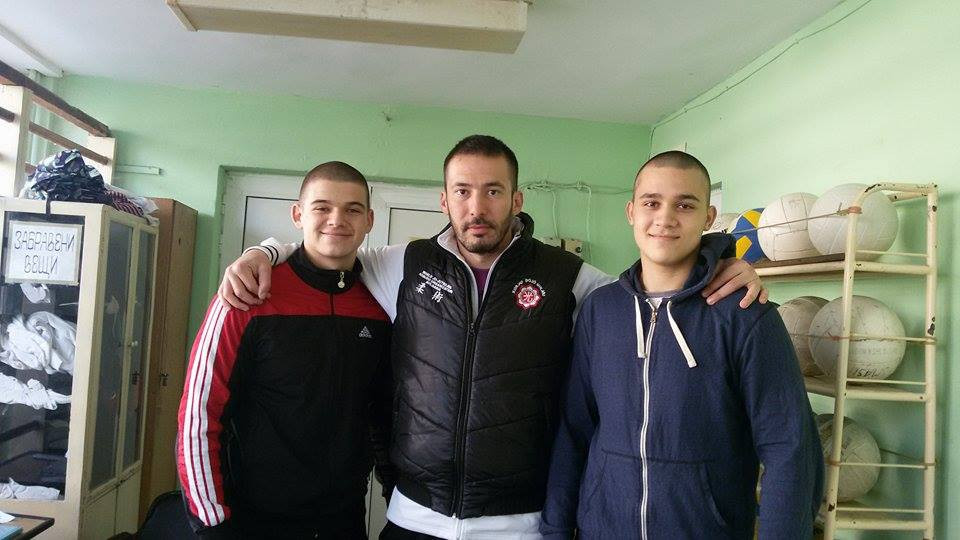
\includegraphics[width=5.1in]{./Aslan/Aslan.jpg},] \end{window}

\begin{center}
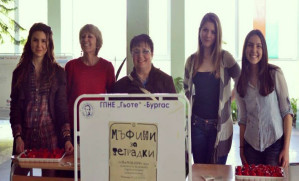
\includegraphics[width=3.1in]{./Komenski/1.jpg} \quad 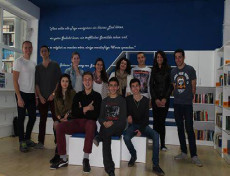
\includegraphics[width=3.1in]{./Komenski/2.jpg} \\
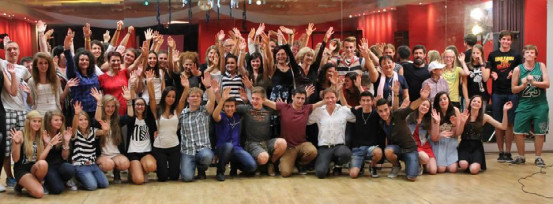
\includegraphics[width=5.1in]{./Komenski/3.jpg}
\end{center}

 
\closearticle


